\section{curve-add}
\label{curve-add}

Take curve-secp256k1 as example, the same as other texs.

\begin{enumerate}
    \item target
        implement the addition of two different curve points. this is a incomplete addition, you can refer to The halo2 Book \cite{website:halo2-book} to learn more about it.
    \item constraints-logic
        \begin{figure}[!ht]
            \centering
            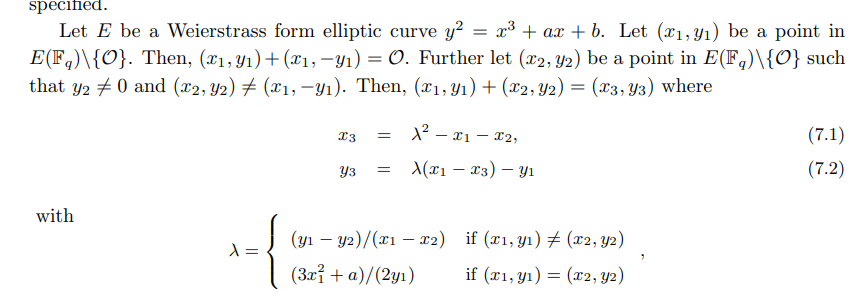
\includegraphics[width=0.8\textwidth]{curve-add.jpg}
            \caption{curve-add}
            \label{fig:curve-add}
        \end{figure}
    \item curve-add process layout
        \begin{figure}[!ht]
            \centering
            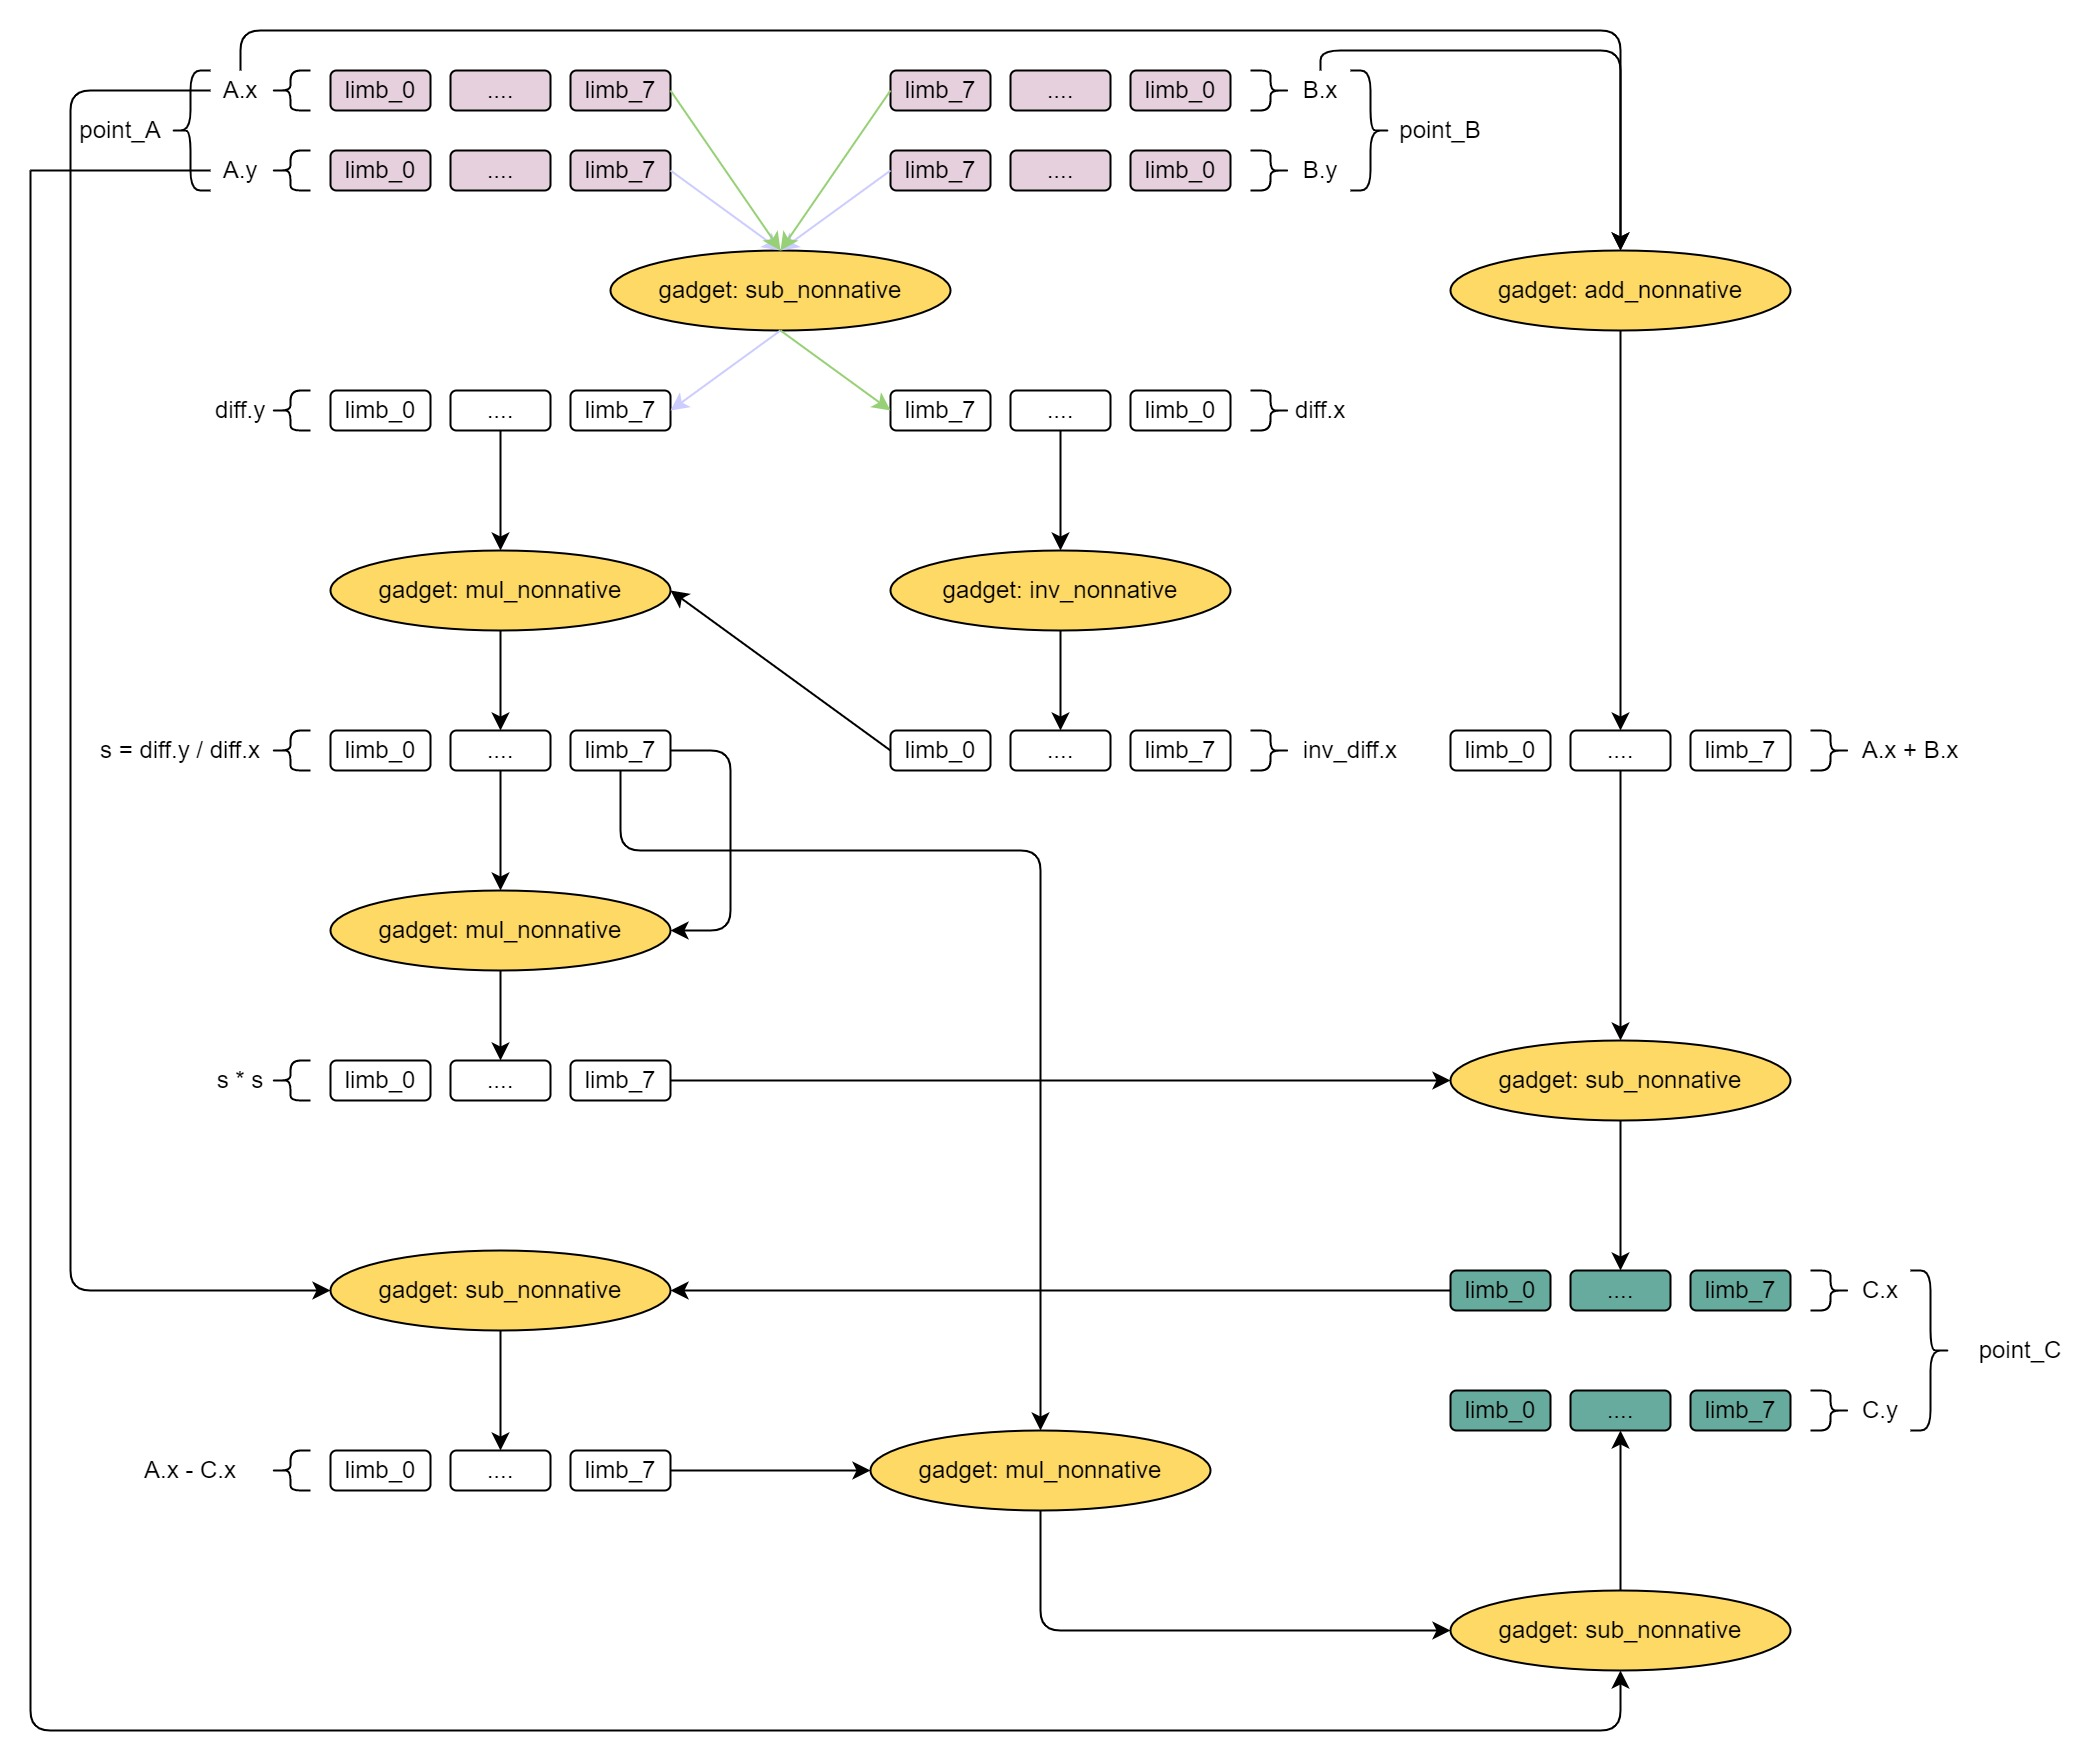
\includegraphics[width=0.8\textwidth]{curve-add-layout.jpg}
            \caption{curve-add layout}
            \label{fig:curve-add-layout}
        \end{figure}
    
    \item constraints-info and costs
        \begin{itemize}
            \item gadget-sub-nonnative num: 5
            \item gadget-add-nonnative num: 1
            \item gadget-mul-nonnative num: 3
            \item gadget-inv-nonnative num: 1
            \item gate type num: 
            \item gate instance num: 
        \end{itemize}

\end{enumerate}